\chapter{Postprocessing\label{chapter:FEM}}
\begin{chapquote}{Gerhard K\"onig%, \textit{\url{https://en.wikiquote.org/wiki/Albert_Einstein}}
	}
	``The source of mistake is always between the keyboard and the chair. So, check, double check and check again.''
\end{chapquote}
\section{Rigorous Methods}
In the following, we will introduce some widely used post-processing methods. Each method has its pros-and-cons. For comparison of these methods, please refer to some benchmark papers.\cite{ShirtsJCP2005,YtrebergJCP2006,PaliwalJCTC2011} 
% !TeX spellcheck = en_US
\subsection{Thermodynamic Perturbation\label{Sec:FEM:TP}}
Thermodynamic Perturbation (TP), also known as Free Energy Perturbation (FEP), exponential average, or Zwanzig equation was developed by Zwanzig.\cite{ZwanzigJCP1954}. 

A reference system containing N-particles can be described by Hamiltonian $H_{0}(\textbf{x},\textbf{p}_{x})$, which is a function of 3N Cartesian coordinates, $\textbf{x}$, and their conjugated momenta, $\textbf{p}_{x}$. The target system similarly can be described by the Hamiltonian $H_{1}(\textbf{x},\textbf{p}_{x})$. Both the two systems can be connected by 
\begin{equation}
H_{1}(\textbf{x},\textbf{p}_{x}) = H_{0}(\textbf{x},\textbf{p}_{x}) + \Delta H (\textbf{x},\textbf{p}_{x})
\label{Eq:deltaH}
\end{equation}
The Helmholtz free energy difference between the target and the reference systems, $\Delta A$, can be given in terms od the ratio of the corresponding partition functions, $Q_{1}$ and $Q_{0}$:
\begin{equation}
\Delta A  =  -\frac{1}{\beta}ln\frac{Q_{1}}{Q_{0}},
\label{Eq:deltaA}
\end{equation}
where $\beta = {(k_{B}T)}^{-1}$, and
\begin{equation}
Q = \frac{1}{{h}^{3N}N!} \int\int \exp[-\beta H(\textbf{x},\textbf{p}_{x})] d\textbf{x}d\textbf{p}_\textbf{x},
\label{Eq:PF}
\end{equation}
So, we obtain
\begin{align}
\Delta A  =&  -\frac{1}{\beta}ln\frac{\int\int \exp[-\beta H_{1}(\textbf{x},\textbf{p}_{x}) ] d\textbf{x}d\textbf{p}_\textbf{x}}{\int\int \exp[-\beta H_{0}(\textbf{x},\textbf{p}_{x}) ] d\textbf{x}d\textbf{p}_\textbf{x}} \\
=& -\frac{1}{\beta}ln\frac{\int\int \exp[-\beta \Delta H(\textbf{x},\textbf{p}_{x})] \exp[-\beta H_{0}(\textbf{x},\textbf{p}_{x}) ] d\textbf{x}d\textbf{p}_\textbf{x}}{\int\int \exp[-\beta H_{0}(\textbf{x},\textbf{p}_{x}) ] d\textbf{x}d\textbf{p}_\textbf{x}},
\label{Eq:deltaA2}
\end{align}
The probability density function of finding the reference system in a state defined by positions $\textbf{x}$ and momenta $\textbf{p}_{x}$ is 
\begin{equation}
P_{0}(\textbf{x},\textbf{p}_{x}) = \frac{ \exp[-\beta H_{0}(\textbf{x},\textbf{p}_{x}) ] }{\int\int \exp[-\beta H_{0}(\textbf{x},\textbf{p}_{x}) ] d\textbf{x}d\textbf{p}_\textbf{x}}
\label{Eq:proden}
\end{equation}
If the probability density function is used, the Eq.~\ref{Eq:deltaA2}  becomes
\begin{equation}
\Delta A = -\frac{1}{\beta} \int\int \exp[-\beta \Delta H(\textbf{x},\textbf{p}_{x})] P_{0}(\textbf{x},\textbf{p}_{x}) d\textbf{x}d\textbf{p}_\textbf{x},
\label{Eq:deltaA3}
\end{equation}
or, equivalently,
\begin{equation}
\Delta A = -\frac{1}{\beta} ln \left \langle \exp[-\beta \Delta H(\textbf{x},\textbf{p}_{x})] \right \rangle  _{0},
\label{Eq:deltaA4}
\end{equation}
Here, $\left \langle \cdots \right \rangle _{0}$ denotes an ensemble average over configurations sampled from the reference state. Equation~\ref{Eq:deltaA4} is the basic equation of \textbf{TP}. It states that $\Delta A$ can be estimated by sampling only equilibrium configurations of the reference state.

Note that integration over the kinetic term in the partition function, Eq.~\ref{Eq:PF}, can be carried out analytically. Thus, it cancels out in Eq.~\ref{Eq:deltaA}, and Eq.~\ref{Eq:deltaA4} becomes
\begin{equation}
\Delta A = -\frac{1}{\beta} ln \left \langle \exp(-\beta \Delta U) \right \rangle  _{0},
\label{Eq:deltaA5}
\end{equation}
where $\Delta U$ is the difference in the potential energy between the target and the reference states. The integration implied by the statistical average is now carried out over particle coordinates only.

If we reverse the reference and the target systems, and repeat the same derivation, using the same convention for  $\Delta A$ and $\Delta U$ as before, we obtain
\begin{equation}
\Delta A = \frac{1}{\beta} ln \left \langle \exp(\beta \Delta U) \right \rangle  _{1},
\label{Eq:deltaA6}
\end{equation}
Although expressions Eq.~\ref{Eq:deltaA5} and Eq.~\ref{Eq:deltaA6} are formally equivalent, their convergence properties may be quite different. This means that there is a preferred direction to carry out the required transformation between the two states. One should be start the perturbation from the system having the larger important phase space region. This means that the reference system should be that with the higher entropy, and the transformation should be proceed in the direction in which the entropy change $\Delta S$ is negative. 

The formulas for free energy difference, Eq.~\ref{Eq:deltaA5} and Eq.~\ref{Eq:deltaA6}, are formally exact for any perturbation. However, this does not means that they can always be successfully applied. Since $\Delta A$ is calculated as the average over a quantity that depends only on $\Delta U$, this average can be taken over probability distribution $P_0(\Delta U)$ instead of $P_{0}(\textbf{x},\textbf{p}_{x})$. Then, $\Delta A$ in Eq.~\ref{Eq:deltaA3} can be expressed ad a one dimensional integral over energy difference
\begin{equation}
\Delta A = -\frac{1}{\beta} \int \exp(-\beta \Delta U) P_{0}(\Delta U) d\Delta U,
\label{Eq:deltaA7}
\end{equation}
If $U_{0}$ and $U_{1}$ were the functions of a sufficient number of identically distributed random variable, then $\Delta U$ would be Gaussian distribution, which is a consequence of the central limit theorem. In practice, the probability distribution $P_{0}(\Delta U)$ deviates somewhat from the ideal Gaussian case, but still has a ``Gaussian-like'' shape. This indicates that the value of the integral in Eq.~\ref{Eq:deltaA7} depends on the low-energy tail of the distribution.

Even though $P_{0}(\Delta U)$ is only rarely an exact Gaussian, it is instructive to consider this case in more detail. If we substitute
\begin{equation}
P_{0}(\Delta U) = \frac{1}{\sqrt{2\pi}\sigma}\exp[-\frac{(\Delta U - \left \langle \Delta U \right \rangle_{0})^2}{2\sigma^2}]
\label{Eq:gaussian}
\end{equation}
where
\begin{equation}
\sigma^2 = \left \langle \Delta U^2 \right \rangle_{0} - \left \langle \Delta U \right \rangle_{0}^2
\label{Eq:variance}
\end{equation}
to Eq.~\ref{Eq:deltaA7}, we obtain
\begin{equation}
\exp(-\beta \Delta A) = \frac{C}{\sqrt{2\pi}\sigma} \int \exp[-\frac{(\Delta U - \left \langle \Delta U \right \rangle_{0} - \beta \sigma ^2)^2}{2\sigma^2}] d\Delta U
\label{Eq:expdeltaA}
\end{equation}
Here, $C$ is independent of $\Delta U$
\begin{equation}
C = \exp [-\beta (\left \langle \Delta U \right \rangle_{0} - \frac{1}{2} \beta \sigma ^2)]
\label{Eq:C}
\end{equation}
If $P_{0}(\Delta U)$ is Gaussian, there is, of course, no reason to carry out a numerical integration, since the integral in Eq.~\ref{Eq:expdeltaA} can be evaluated analytically. This yields
\begin{equation}
\Delta A = \left \langle \Delta U \right \rangle_{0} - \frac{1}{2} \beta \sigma ^2
\label{Eq:deltaA8}
\end{equation}
\clearpage 
\subsection{Thermodynamic Integration\label{Sec:FEM:TI}}
Thermodynamic Integration (TI) method was proposed by Kirkwood.\cite{KirkwoodJCP1935}. If the free energy, $A$, is a continuous function of $\lambda$, the free energy difference between two states corresponding to $\lambda=0$ and $\lambda=1$ can be computed via
\begin{equation}
\Delta A = \int_{0}^{1} \frac{\partial{A(\lambda)}}{\partial{\lambda}} \diff\lambda.
\label{Eq:FEM:TI:deltaA1TI}
\end{equation} 
With
\begin{equation}
A(\lambda) = -\beta^{-1}\ln Q(\lambda),
\label{Eq:FEM:TI:Alambda}
\end{equation} 
the partial derivative can be expressed as
\begin{align}
\frac{\partial{A(\lambda)}}{\partial{\lambda}} =& -\beta^{-1} \left[ \frac{\partial{\ln{Q(\lambda)}}}{\partial{\lambda}} \right] \notag\\
=&-\frac{\beta^{-1}}{Q(\lambda)}\frac{\partial{Q(\lambda)}}{\partial{\lambda}}.
\label{Eq:FEM:TI:deltaA2TI}
\end{align} 
From the definition of $Q$
\begin{equation}
Q_{NVT}(\lambda) = \frac{1}{{h}^{3N}N!} \iint \exp[-\beta H(\mathbf{x},\mathbf{p}_{x},\lambda)] \diff\mathbf{x}\diff\mathbf{p}_\mathbf{x},
\label{Eq:FEM:TI:PFTI}
\end{equation}
we have
\begin{align}
\frac{\partial{Q(\lambda)}}{\partial{\lambda}} =&\frac{1}{{h}^{3N}N!} \iint \frac{\partial}{\partial{\lambda}}\exp[-\beta H(\mathbf{x},\mathbf{p}_{x},\lambda)] \diff\mathbf{x}\diff\mathbf{p}_\mathbf{x}\notag\\
=& -\frac{\beta}{{h}^{3N}N!} \iint \frac{\partial{H(\mathbf{x},\mathbf{p}_{x},\lambda)}}{\partial{\lambda}}\exp[-\beta H(\mathbf{x},\mathbf{p}_{x},\lambda)] \diff\mathbf{x}\diff\mathbf{p}_\mathbf{x}.
\label{Eq:FEM:TI:PPF2}
\end{align}
Substituting back into the expression for $\partial{A}/\partial{\lambda}$ yields
\begin{align}
\frac{\partial{A(\lambda)}}{\partial{\lambda}} =& \frac{1}{{h}^{3N}N!}\frac{1}{Q(\lambda)} \iint \frac{\partial{H(\mathbf{x},\mathbf{p}_{x},\lambda)}}{\partial{\lambda}}\exp[-\beta H(\mathbf{x},\mathbf{p}_{x},\lambda)] \diff\mathbf{x}\diff\mathbf{p}_\mathbf{x}, \notag\\
=& \frac{1}{{h}^{3N}N!}\iint \frac{\partial{H(\mathbf{x},\mathbf{p}_{x},\lambda)}}{\partial{\lambda}}\cdot\frac{\exp[-\beta H(\mathbf{x},\mathbf{p}_{x},\lambda)]}{Q(\lambda)} \diff\mathbf{x}\diff\mathbf{p}_\mathbf{x},\notag \\
=& \left \langle \frac{\partial{H(\mathbf{x},\mathbf{p}_{x}, \lambda)}}{\partial{\lambda}} \right \rangle_{\lambda}
\label{Eq:FEM:TI:PA2}
\end{align}
Thus, the basic TI formula is
\begin{equation}
\Delta A = \int_{\lambda=0}^{\lambda=1}\left \langle \frac{\partial{H(\mathbf{x},\mathbf{p}_{x},\lambda)}}{\partial{\lambda}} \right \rangle_{\lambda} \diff\lambda
\label{Eq:FEM:TI:TI}
\end{equation} 
where $\left \langle \cdots \right \rangle _{\lambda}$ corresponds to the ensemble average obtained using the Hamiltonian $H(\lambda)$. In practice, the ensemble of configurations can be obtained by molecular dynamics or Monte Carlo simulations. It is common practice in free energy calculations to use the coupling parameter $\lambda$ for defining the transformation from the initial state $A$ with Hamiltonian $H_{A}$ to the final state $B$ with Hamiltonian $H_{B}$. The simplest coupling is linear transformation as
\begin{equation}
H(\lambda) = (1-\lambda) H_{A} + \lambda H_{B}
\end{equation}
The accuracy of TI integral formula depends on the exactness of the numerical integration method.\cite{PaliwalJCTC2011} Practically, the integrand in Eq.~\ref{Eq:FEM:TI:TI} needs to be evaluated over a number of discrete points $\lambda_{i}$, and then be summed up to give the free energy difference between $\lambda=0$ and $1$, for instance via the trapezoidal rule
\begin{equation}
\Delta A = \sum_{i=0}^{N-1}\frac{1}{2}\left(\left \langle \frac{\partial{H(\lambda)}}{\partial{\lambda}} \right \rangle_{\lambda_{i}} + \left \langle\frac{\partial{H(\lambda)}}{\partial{\lambda}} \right \rangle_{\lambda_{i+1}}\right)
(\lambda_{i+1}-\lambda_i).
\label{Eq:FEM:TI:dTI}
\end{equation} 
A finite number of $\lambda_{i}$ values between 0 and 1 are chosen and for each of them a complete molecular dynamics simulation is carried out resulting in an ensemble of configurations generated with $H(\lambda_{i})$.
The ensemble average of the derivative of the Hamiltonian with respect to $\lambda$ is then calculated for each $\lambda_{i}$.
	
In addition to summation method, the simplest numerical integration is to evaluate the integrand at the midpoint:
\begin{equation}
\Delta A \simeq \left \langle \frac{\partial{H(\lambda)}}{\partial{\lambda}} \right \rangle_{\lambda=\frac{1}{2}}
\label{Eq:FEM:TI:TI1}
\end{equation} 
This might be a good first thing to do to get some impression of what is going on, but is only accurate for very smooth or small changes. %Gaussian quadrature formulas of higher order are generally more useful:
%\begin{equation}
%\Delta A = \sum_{i}^{} w_{i}\left \langle \frac{\partial{H(\lambda)}}{\partial{\lambda}} \right \rangle_{\lambda_{i}}
%\label{Eq:FEM:TI:Gauss}
%\end{equation} 
%Some weights and quadrature points are given in the table~\ref{tab:Gauss}; other formulas are possible, \cite{HummerJCP1996} but the Gaussian one listed here are probably the most useful. The formulas are always symmetrical about $\lambda = 0.5$, so that $\lambda$ and $(1-\lambda)$ both have the same weight.
	
%\clearpage
%\begin{table*}
%	\caption{\label{tab:Gauss}Abscissas and weights for Gaussian integration.}
%	\newcommand{\rb}[1]{\raisebox{1.5ex}[0t]{#1}}
%	\begin{tabular}{lcccccccccccccccccc}
%		\hline
%	   n&$\lambda_{i}$&$1-\lambda_{i}$&$w_{i}$ \\
%		\hline
%	   1&     0.5&        & 1.0 \\
%		\hline
%	   2& 0.21132& 0.78867& 0.5 \\
%		\hline
%	   3&  0.1127& 0.88729& 0.27777 \\
%		&     0.5&        & 0.44444 \\
%		\hline
%	   5& 0.04691& 0.95308& 0.11846 \\
%		& 0.23076& 0.76923& 0.23931 \\
%		&     0.5&        & 0.28444 \\
%		\hline
%	   7& 0.02544& 0.97455& 0.06474 \\
%		& 0.12923& 0.87076& 0.13985 \\
%		& 0.29707& 0.70292& 0.19091 \\
%		&     0.5&        & 0.20897 \\
%		\hline
%	   9& 0.01592& 0.98408& 0.04064 \\
%		& 0.08198& 0.91802& 0.09032 \\
%		& 0.19331& 0.80669& 0.13031 \\
%		& 0.33787& 0.66213& 0.15617 \\
%		&     0.5&        & 0.16512 \\
%		\hline
%	  12& 0.00922& 0.99078& 0.02359 \\ 
%		& 0.04794& 0.95206& 0.05347 \\
%		& 0.11505& 0.88495& 0.08004 \\
%		& 0.20634& 0.79366& 0.10158 \\
%		& 0.31608& 0.68392& 0.11675 \\
%		& 0.43738& 0.56262& 0.12457 \\
%		\hline
%	\end{tabular} 
%\end{table*}
\clearpage
% !TeX spellcheck = en_US
\subsection{Bennett Acceptance Ratio\label{Sec:FEM:BAR}}
\begin{chapquote}{Professor Savas Dimopoulos, Stanford University}
	``The thing that differentiates scientists is purely an artistic ability to discern what is a good idea, what is a beautiful idea, what is worth spending time on, and most importantly, what is a problem that is sufficiently interesting, yet sufficiently difficult, that is hasn't yet been solved, but the time for solving it has come now.''
\end{chapquote}
Bennett acceptance ratio was developed by Bennett in 1976,\cite{BennettJComputPhys1976} and was re-discovered by Crooks\cite{CrooksPRE2000} for Markovian and balanced dynamics and by Shirts et al\cite{ShirtsPRL2003} using maximum likelihood over 20 years later. The Metropolis function is defined as
\begin{equation}
	M(x)=min\{1,\exp{(-x)}\},
\end{equation}
which has the property 
\begin{equation}
	M(x)/M(-x)=\exp{(-x)}.
\end{equation}

If we make a trial move that keeps the same configuration ($q_{1},\cdots,q_{N}$)
but switches the potential function from $U_{0}$ to $U_{1}$ or vice-versa, 
the acceptance probabilities for such a pair of trial moves must satisfy
the detailed balance
\begin{equation}
	M(U_{1}-U_{0})\exp{(-U_{0})}=M(U_{0}-U_{1})\exp{(-U_{1})}.
\end{equation}

Integrating this identity over all of configuration space and multiplying
by the trivial factors $Q_{0}/Q_{0}$ and $Q_{1}/Q_{1}$, one obtains:

\begin{equation}
	Q_{0}\frac{\displaystyle\int M(U_{1}-U_{0})\exp{(-U_{0})}\diff\mathbf{{q}}}{Q_{0}}=Q_{1}\frac{\displaystyle\int M(U_{0}-U_{1})\exp{(-U_{1})}\diff\mathbf{{q}}}{Q_{1}},
\end{equation}
or simply

\begin{equation}
	\frac{Q_{0}}{Q_{1}}=\frac{\langle M(U_{0}-U_{1})\rangle_{1}}{\langle M(U_{1}-U_{0})\rangle_{0}}.\label{eq:FEM:BAR:MetropolisRatio}
\end{equation}

The physical meaning of this formula is that a Monte Carlo calculation
that includes potential-switching trial moves would distribute configurations
between $U_{1}$ and $U_{0}$ in the ratio of their configurational
integrals. 

A formula more general than Eq.~\ref{eq:FEM:BAR:MetropolisRatio} can be written as
\begin{equation}
	\frac{Q_{0}}{Q_{1}}=\frac{Q_{0}}{Q_{1}}\frac{\displaystyle\int W\exp{(-U_{0}-U_{1})}\diff\mathbf{{q}}}{\displaystyle\int W\exp{(-U_{1}-U_{0})}\diff\mathbf{{q}}}=\frac{\langle W\exp{(-U_{0})}\rangle_{1}}{\langle W\exp{(-U_{1})}\rangle_{0}},\label{eq:FEM:BAR:weightedratio}
\end{equation}
where $W$ is an arbitrary weighting function.

Optimization of the free energy estimate is most easily carried out in the limit of large sample sizes. Let the available data consist
of $n_{0}$ statistically independent configurations from the $U_{0}$ ensemble and $n_{1}$ from the $U_{1}$ ensemble, and let the data
be used in Eq.~\ref{eq:FEM:BAR:weightedratio} to obtain a finite-sample estimate of the reduced free energy difference $\Delta A=A_{1}-A_{0}=\ln{(Q_{0}/Q_{1})}$.
Using the error propagation law of uncorrelated variables ($covar(x_1,x_2)=0$),\cite{BerendsenBook2011}
\begin{equation}
	\delta^2\left[y(x_{1},x_{2})\right]=\left(\frac{\partial y}{\partial x_{1}}\right)^{2}\delta^2(x_{1})+\left(\frac{\partial y}{\partial x_{2}}\right)^{2}\delta^2(x_{2}).
\end{equation}

Thus we have the variance of $\Delta A$
\begin{eqnarray}
	\delta^2(\Delta A) & = & \left(\frac{\partial\Delta A}{\partial Q_{0}}\right)^{2}\delta^2Q_0+\left(\frac{\partial\Delta A}{\partial Q_{1}}\right)^{2}\delta^2Q_1\notag\\
	& = & \left(\frac{1}{Q_{0}}\right)^{2}\delta^2Q_0+\left(-\frac{1}{Q_{1}}\right)^{2}\delta^2Q_1\notag\\
	& = & \left(\frac{1}{Q_{0}}\right)^{2}\delta^2Q_0+\left(\frac{1}{Q_{1}}\right)^{2}\delta^2Q_1.
\end{eqnarray}

With the definition of variance $\delta^2X=\left\langle X^{2}\right\rangle -\left\langle X\right\rangle ^{2}$,
we have 
\begin{eqnarray}
	\delta^2Q_0 & = & \delta^2\left\langle W\exp{(-U_{0})}\right\rangle_{1}\notag\\
	& = & \delta^2\left(\frac{1}{n_1}\sum_{i=1}^{n_1}W_{i}\exp{\left(-U_{0}(i)\right)}\right)\notag\\
	& = & \sum_{i=1}^{n_{1}}\left(\frac{1}{n_{1}}\right)^{2}\delta^2\left(W_{i}\exp{\left(-U_{0}(i)\right)}\right)\notag\\
	& = & \frac{1}{n_{1}}\delta^2\left(W_{i}\exp{\left(-U_{0}(i)\right)}\right)\notag\\
	& = & \frac{1}{n_{1}}\left\{ \left< \left[W\exp{(-U_{0})}\right]^{2}\right>_{1}-\left[\left< W\exp{(-U_{0})}\right>_{1}\right]^{2}\right\}\notag\\
	& = & \frac{1}{n_{1}}\left\{ \left< W^{2}\exp{(-2U_{0})}\right>_{1}-\left[\left< W\exp{(-U_{0})}\right>_{1}\right]^{2}\right\},
\end{eqnarray}
which shows that the variance of the mean of the samples equals to the variance of the samples divided by the number of samples.

With sufficiently large sample sizes, the error of this estimate will
be nearly Gaussian, and its expected square is exactly the variance
of $\Delta A$ 
\begin{align}
	\delta^2 & (\Delta A_{est}-\Delta A)\nonumber \\
	\approx & \frac{\langle W^{2}\exp{(-2U_{1})}\rangle_{0}}{n_{0}[\langle W\exp{(-U_{1})}\rangle_{0}]^{2}}+\frac{\langle W^{2}\exp{(-2U_{0})}\rangle_{1}}{n_{1}[\langle W\exp{(-U_{0})}\rangle_{1}]^{2}}-\frac{1}{n_{0}}-\frac{1}{n_{1}}\nonumber \\
	= & \frac{\displaystyle\int\left[\frac{Q_{0}}{n_{0}}\exp{(-U_{1})}+\frac{Q_{1}}{n_{1}}\exp{(-U_{0})}\right]W^{2}\exp{(-U_{0}-U_{1})}\diff\mathbf{q}}{\left[\displaystyle\int W\exp{(-U_{0}-U_{1})}\diff\mathbf{q}\right]^{2}}\notag\\
	  &-\frac{1}{n_{0}}-\frac{1}{n_{1}}.\label{eq:FEM:BAR:expectation}
\end{align}

To minimize it with respect to $W$, we have
\begin{equation}
	W=const\times\left(\frac{Q_{0}}{n_{0}}\exp{(-U_{1})}+\frac{Q_{1}}{n_{1}}\exp{(-U_{0})}\right)^{-1}.
	\label{eq:FEM:BAR:W}
\end{equation}

Substituting this into Eq.~\ref{eq:FEM:BAR:weightedratio} yields
\begin{equation}
	\frac{Q_{0}}{Q_{1}}=\frac{\langle f(U_{0}-U_{1}+C)\rangle_{1}}{\langle f(U_{1}-U_{0}-C)\rangle_{0}}\exp{(+C)},
	\label{Eq:FEM:BAR:BAR}
\end{equation}
where
\begin{equation}
	C=\ln\frac{Q_{0}n_{1}}{Q_{1}n_{0}},
	\label{Eq:FEM:BAR:C}
\end{equation}
and $f$ denotes the Fermi function
\begin{equation}
	f(x)=\frac{1}{1+\exp{(+x)}}.
\end{equation}
It can also be expressed as\cite{ShirtsPRL2003}
\begin{equation}
	n_1\langle f(U_{0}-U_{1}+C)\rangle_{1}=n_0\langle f(U_{1}-U_{0}-C)\rangle_{0}.
\end{equation}
It should be noted that Eq.~\ref{Eq:FEM:BAR:BAR} is true for any $C$, which is actually a shift for one of the potential function. But the particular value specified in Eq.~\ref{Eq:FEM:BAR:C} minimizes the expected square error given the finite numbers ($n_0$ and $n_1$) of samples.

The variance of $\Delta A$ can be obtained by substituting Eq.~\ref{eq:FEM:BAR:W} into Eq.~\ref{eq:FEM:BAR:expectation}, and is 
\begin{align}
	\delta^2 \Delta A =&\frac{\left<f^2(U_{1}-U_{0}-C)\right>_0}{n_0\left<f(U_{1}-U_{0}-C)\right>_0^2}+\frac{\left<f^2(U_{0}-U_{1}+C)\right>_1}{n_1\left<f(U_{0}-U_{1}+C)\right>_1^2}-\frac{1}{n_0}-\frac{1}{n_1}\notag\\
	=&\left(\int \frac{n_0n_1\rho_0\rho_1}{n_0\rho_0+n_1\rho_1}\diff \mathbf{q}\right)^{-1}-\frac{n_0+n_1}{n_0n_1},
\end{align}
in which $\rho_i=\exp{(-U_i)}/Q_i$ is the probability.

It is worth emphasizing that Bennett acceptance ratio is asymptotically unbiased, and no other asymptotically unbiased estimator has lower asymptotic mean-squared error. However, it is not clear whether its behavior is always better than other estimators with finite sample sizes.

Shirts et al showed that BAR can be interpreted in terms of the maximum likelihood estimate of the free energy difference given a set of work values in the forward and reverse directions.\cite{ShirtsPRL2003} Starting from (refer to Appendix~\ref{chapter:Appendix:DeltaUDistributions} for the proof)
\begin{equation}
	\ln\left[\frac{P(W|F)}{P(-W|R)}\right]=\beta (W-\Delta F),
	\label{eq:FEM:BAR:distributionratio}
\end{equation}
where $P(W|F)$ ($P(W|R)$) is probability distribution for the work from the two states in the forward (reverse) direction, which can also be thought as the conditional probability of a work value given that it is a forward (reverse) measurement. To simplify the notation, the work $W$ from the reverse direction will be replaced by $-W$. Using the fact that $P(F|W)+P(R|W)=1$, the ratio can be rewritten as
\begin{equation}
	\frac{P(W|F)}{P(R|R)}=\frac{P(F|W)P(R)}{P(R|W)P(F)}=\frac{P(F|W)}{1-P(F|W)}\frac{P(R)}{P(F)}.
\end{equation}
It can be realized that $P(R)/P(F)=n_R/n_F$, where $n_F$ ($n_R$) is the number of forward (reverse) measurement. Defining $M=\ln{n_F/n_R}$, Eq.~\ref{eq:FEM:BAR:distributionratio} can be rewritten as
\begin{equation}
	\ln\frac{P(F|W)}{1-P(F|W)}=(M+W-\Delta F),
\end{equation}
which leads to
\begin{align}
	P(F|W_i)=&\frac{1}{1+\exp[-(M-W_i-\Delta F)]},\\
	P(R|W_i)=&\frac{1}{1+\exp[M-W_i-\Delta F]}
\end{align}
for a single work measurement $W_i$, given a value of the free energy difference $\Delta F$.

Given a value for $\Delta F$, the overall likelihood $L$ becomes
\begin{equation}
	L(\Delta F)=\prod_{i=1}^{n_F}P(F|W_i)\prod_{i=1}^{n_R}P(R|W_i).
\end{equation}
The most likely value of $\Delta F$ is the value that maximizes the (log) likelihood, therefore we have
\begin{align}
	0=\frac{\partial \log L(\Delta F)}{\partial \Delta F}=&-\sum_{i=1}^{n_F}\frac{1}{1+\exp\left[M+W_i-\Delta F\right]}\notag\\
	                                                      &+\sum_{j=1}^{n_R}\frac{1}{1+\exp\left[-(M+W_j-\Delta F)\right]},
\end{align}
which equivalent to the BAR method.
\clearpage 
% !TeX spellcheck = en_US
\subsection{Weighted Histogram Analysis Method\label{Sec:FEM:WHAM}}
The weighted histogram analysis method is a generalization of the histogram method developed by Ferrenberg and Swendsen.\cite{FerrenbergPRL1989}
\subsubsection{Weighted Histogram Analysis Method for Parallel Tempering\label{Sec:FEM:WHAM_REMD}}
The following derivation quite follows Ref.~\cite{ChoderaJCTC2007}.
The central quantity in statistical mechanics is partition function $Z$, which in textbook is often written as
\begin{equation}
Z=\int \exp{-\beta U(\mathbf{R})}d\mathbf{R}.
\end{equation}
This is an integral in coordinate space. It also can be written as an integral in energy space
\begin{equation}
Z=\int \Omega(U)\exp{(-\beta U)}dU,
\end{equation}
where $\Omega(U)$ is density of states and $\Omega(U)\Delta U$ is the number of states in the region $U-\Delta U/2<U<U+\Delta U/2$. Accordingly, the statistical expectation of an operator $\mathbf{A}$ can be calculated by
\begin{equation}
\langle \mathbf{A}\rangle=\frac {\int \mathbf{A}(U)\Omega(U)\exp{(-\beta U)}dU}{\int \Omega(U)\exp{(-\beta U)}dU},
\end{equation}
where
\begin{equation}
\mathbf{A}(U^\prime)=\frac{\int \delta (U(\mathbf{R})-U^\prime)A(\mathbf{R})d\mathbf{R}}{\int \delta (U(\mathbf{R})-U^\prime)d\mathbf{R}}.
\end{equation}
Therefore, the core objective is to calculate $\Omega(U)$.

Suppose we have one trajectory with $N$ snapshots denoted as $\{\mathbf{R}_n\}$. We then discretize the energy space into $M$ bins with width $\Delta U$, and count the number of snapshots fallen into each bin. For convenience, we define $\psi_m(U)$ as
\begin{equation}
	\psi_m(U)= 
	\left\{ 
	\begin{array}{rl} 
	1 & if\,U\in \left[ U_m-\Delta U/2, U_m+\Delta U/2\right)\\ 
	0 & otherwise\\  
	\end{array} 
	\right. 
\end{equation}
Then the histogram for the m$\mathit{th}$ energy bin is
\begin{equation}
	H_{m}=\sum\limits_{n=1}^{N}\psi_{m}(U(\mathbf{R}_n))=N\cdot \frac 1 N\sum\limits_{n=1}^{N}\psi_{m}(U(\mathbf{R}_n))=N\cdot\left<\psi_m\right>,
\end{equation}
with variances (see Appendix~\ref{chapter:Appendix:Uncertainty})
\begin{align}
	\delta^2 H_m=&N^2\delta^2(\left<\psi_m\right>)\notag\\
	            =&g_m N\left(\left<{\psi_m}^2\right>-\left<\psi_m\right>^2\right)\notag\\
	            =&g_m N\left(\left<\psi_m\right>-\left<\psi_m\right>^2\right)\notag\\
	            =&g_m\left<H_m\right>\left(1-\frac{\left<H_m\right>}{N}\right).
\end{align}

A sample histogram in 2D space is shown in Fig.~\ref{Fig:FEM:WHAM:histogram}.
\begin{figure}[htbp]
	\centering
	\includegraphics[width=0.8\textwidth]{figures/histogram.pdf}\\
	\caption{A sample histogram in 2D space, for instance potential energy and a reaction coordinate $\xi$.}\label{Fig:FEM:WHAM:histogram}
\end{figure}

The ratio of the histogram $H_m$ to the total number of snapshots $N$ divided by the bin width $\Delta U$ can be approximately taken as the probability of states in this bin, i.e.,
\begin{equation}
	\frac{\Omega_m\exp{(-\beta U_m)}}{Z}\approx\frac{H_m}{N\Delta U}.
\end{equation}
Therefore,
\begin{align}
	\Omega_m=&\frac{1}{\Delta U}\cdot\frac{H_m}{N}\cdot\frac{Z(\beta)}{\exp{(-\beta U_m)}}\notag\\
	        =&\frac{H_m}{N\Delta U\exp{\left[f_k-\beta_kU_m\right]}},
	\label{Eq:FEM:WHAM:DoSsingle}
\end{align}
and variances
\begin{equation}
	\delta^2\Omega_m=\frac{\delta^2 H_m}{\left(N\Delta U\exp{\left[f_k-\beta_kU_m\right]}\right)^2},
\end{equation}
in which we have defined a dimensionless free energy $f=-\ln{Z(\beta)}$.

Practically, we may run multiple ($K$) trajectories using, for example, replica exchange molecular dynamics simulations. For each trajectory (index $k$), we have unique estimators for the histogram $H_{mk}$, the density of states $\Omega_{mk}$ and their variances $\delta^2 H_{mk}$ and $\delta^2\Omega_{mk}$ being
\begin{equation}
	H_{mk}=\sum\limits_{n=1}^{N_k}\psi_{m}(U(\mathbf{R}_{kn})),
\end{equation}
\begin{equation}
	\delta^2 H_{mk}=g_{mk}\left<H_{mk}\right>\left(1-\frac{\left<H_{mk}\right>}{N_k}\right),
\end{equation}
\begin{align}
	\Omega_{mk}=\frac{H_{mk}}{N_k\Delta U\exp{\left[f_k-\beta_kU_{mk}\right]}},
	\label{Eq:FEM:WHAM:Omega_mk}
\end{align}
and
\begin{equation}
	\delta^2\Omega_{mk}=\frac{\delta^2 H_{mk}}{\left(N_k\Delta U\exp{\left[f_k-\beta_kU_{mk}\right]}\right)^2},
\end{equation}
The optimum estimator of the density of states from all the simulations is
\begin{equation}
	\Omega_m=\frac{\sum\limits_{k=1}^K\left[\delta^2\Omega_{mk}\right]^{-1}\Omega_{mk}}{\sum\limits_{k=1}^K\left[\delta^2\Omega_{mk}\right]^{-1}},
	\label{Eq:FEM:WHAM:optimumOmega}
\end{equation}
which is the weighted average of density of states of all the trajectories with the weight reversely proportional to the uncertainties (see Appendix~\ref{chapter:Appendix:Mean}).

To make the expression simpler, here we take some approximations. First, normally the energy space is split into a large number of bins. The histogram in each bin is much smaller than the total number of snapshots, i.e. $H_{mk}\ll N_k$. The average of $H_{mk}$ can be related to the optimum estimator of the density of states, i.e.
\begin{equation}
	\left<H_{mk}\right>=N_k\Delta U\Omega_m\exp{(f_k-\beta_kU_m)}.
\end{equation}
Then we have
\begin{equation}
    \delta^2H_{mk}=g_{mk}N_k\Delta U\Omega_m\exp{(f_k-\beta_kU_m)}
\end{equation}
and
\begin{equation}
\delta^2\Omega_{mk}=\frac{\Omega_m}{{g_{mk}}^{-1}N_k\Delta U\exp{(f_k-\beta_kU_m)}}.
\label{Eq:FEM:WHAM:delta2Omega_mk}
\end{equation}

Taking Eq.~\ref{Eq:FEM:WHAM:Omega_mk} and Eq.~\ref{Eq:FEM:WHAM:delta2Omega_mk} into Eq.~\ref{Eq:FEM:WHAM:optimumOmega}, we find
\begin{equation}
\Omega_m=\frac{\sum\limits_{k=1}^{K}{g_{mk}}^{-1}H_{mk}}{\sum\limits_{k=1}^{K}{g_{mk}}^{-1}N_k\Delta U\exp{(f_k-\beta_kU_m)}},
\label{Eq:FEM:WHAM:Omega_iteration}
\end{equation}
in which
\begin{equation}
f_k=-ln\sum\limits_{m=1}^M\Omega_m\Delta U\exp{(-\beta_kU_m)}.
\label{Eq:FEM:WHAM:f_k_iteration}
\end{equation}
Obviously, Eq.~\ref{Eq:FEM:WHAM:Omega_iteration} and Eq.~\ref{Eq:FEM:WHAM:f_k_iteration} must be solved iteratively.
The uncertainty of $\Omega_m$ is given by
\begin{equation}
\delta^2 \Omega_m=\frac{\Omega_m}{\sum\limits_{k=1}^K{g_{mk}}^{-1}N_k\Delta U\exp{(f_k-\beta_kU_m)}}
\end{equation}
and the relative uncertainty is given by
\begin{equation}
\frac{\delta^2\Omega_m}{\Omega_m^2}=\left[\sum\limits_{k=1}^K{g_{mk}}^{-1}H_{mk}\right]^{-1}.
\end{equation}
Using the density of states and its variance, we can estimate the expectation of any configuration function $A(\mathbf{R})$ at any inverse temperature $\beta$
\begin{equation}
\left<A\right>_\beta\approx\frac{\sum\limits_{m=1}^M\Omega_m\Delta U\exp{(-\beta U_m)}A_m}{\sum\limits_{m=1}^M\Omega_m\Delta U\exp{(-\beta U_m)}},
\label{Eq:FEM:WHAM:A}
\end{equation}
where
\begin{equation}
A_m=\frac{\int d\mathbf{R}A(\mathbf{R})\psi_m(U(\mathbf{R}))}{\int d\mathbf{R}\psi_m(U(\mathbf{R}))}.
\end{equation}
Using histograms of bin $m$ from all the simulations and defining $H_m=\sum\limits_{k=1}^KH_{mk}$, an estimator of $A_m$ denoted as $\hat{A}_m$ can be calculated as
\begin{equation}
   \hat{A}_m={H_{m}}^{-1}\sum\limits_{k=1}^K\sum\limits_{n=1}^{N_k}\psi_m(U(\mathbf{R}_{kn}))A(\mathbf{R}_{kn}).
   \label{Eq:FEM:WHAM:A_m}
\end{equation}
Taking Eq.~\ref{Eq:FEM:WHAM:A_m} into Eq.~\ref{Eq:FEM:WHAM:A}, we obtain an estimator of $\hat{A}(\beta)$
\begin{align}
\hat{A}(\beta)=&\frac{\sum\limits_{m=1}^M\Omega_m\Delta U\exp{(-\beta U_m)}{H_{m}}^{-1}\sum\limits_{k=1}^K\sum\limits_{n=1}^{N_k}\psi_m(U(\mathbf{R}_{kn}))A(\mathbf{R}_{kn})}{\sum\limits_{m=1}^M\Omega_m\Delta U\exp{(-\beta U_m)}}\\
              =&\frac{\sum\limits_{m=1}^M\Omega_m\Delta U\exp{(-\beta U_m)}{H_{m}}^{-1}\sum\limits_{k=1}^K\sum\limits_{n=1}^{N_k}\psi_m(U(\mathbf{R}_{kn}))A(\mathbf{R}_{kn})}{\sum\limits_{m=1}^M\Omega_m\Delta U\exp{(-\beta U_m)}{H_{m}}^{-1}\sum\limits_{k=1}^K\sum\limits_{n=1}^{N_k}\psi_m(U(\mathbf{R}_{kn}))}\\
              =&\frac{\sum\limits_{k=1}^K\sum\limits_{n=1}^{N_k}w_{kn}(\beta)A_{kn}}{\sum\limits_{k=1}^K\sum\limits_{n=1}^{N_k}w_{kn}(\beta)},
\end{align}
where the per-configuration weights $w_{kn}(\beta)$ is given by
\begin{equation}
w_{kn}(\beta)=\sum\limits_{m=1}^M{H_{m}}^{-1}\psi_m(U(\mathbf{R}_{kn}))\Omega_m\exp{(-\beta U_m)}
\end{equation}

\subsubsection{Weighted Histogram Analysis Method From Maximum Likelihood}
The following derivation quite follows Ref.~\cite{GallicchioJPCB2005}, in which maximum likelihood principle is utilized. 
Suppose we have performed $K$ simulations, each at a different inverse temperature $\beta_k$ and possibly with different biasing potential $w_k(\mathbf{R})$.
We then discretize the 2D plane spanned by the coordinate and unbiased potential energy into bins, each characterized by ${\mathbf{R}_j}$ and ${E_h}$. To make the following derivation cleaner, we map the 2D bins to one dimensional series with index $l, l=1,\dots,L$. Next, we construct histograms for bins using all the samples from the simulations. The probability of finding the system in bin $l$ during the $k$th simulation can be written as
\begin{equation}
p_{k,l}=f_kc_{k,l}p_l^0,
\end{equation}
in which $p_l^0$ is the (simulation-independent) unbiased probability,
\begin{align}
c_{k,l}=&\exp{\left\{-\beta_k\left[E_l+w_{k,l}\right]+\beta_0E_l\right\}}\notag\\
       =&\exp{\left[-\left(\beta_k-\beta_0\right)E_l\right]}\exp{\left(-\beta_kw_{i,l}\right)}
\end{align}
is the bias factor, $E_l$ is the unbiased energy of bin $l$, $f_k={\{\sum\limits_lc_{k,l}p_l^0\}}^{-1}$ is the normalization factor.
It is worth emphasizing that the biasing potential can be multiple dimensional as, for instance, in a two-dimensional umbrella sampling.
If the biasing is only in temperature-space as in replica exchange molecular dynamics
\begin{equation}
c_{k,l}=\exp{\left[-\left(\beta_k-\beta_0\right)E_l\right]},
\end{equation} 
while if the biasing is only in potential as in umbrella sampling
\begin{equation}
c_{k,l}=\exp{\left(-\beta_0w_{k,l}\right)}.
\end{equation}

If we assume that each count in each histogram is independent, then the likelihood of observing the $k$th histogram is given by the multinomial distribution
\begin{align}
P(n_{k,1},n_{k,2},\dots,n_{k,L}|p_{k,1},p_{k,2},\dots,p_{k,L})=\notag\\
\frac{\left(\sum\limits_l n_{k,l}\right)!}{\prod\limits_l n_{k,l}!}\prod\limits_{l=1}^L\left(p_{k,l}\right)^{n_{k,l}}\propto\prod\limits_{l=1}^{L}\left(f_kc_{k,l}p_l^0\right)^{n_{k,l}}.
\end{align}
For all $K$ simulations, the likelihood is the product of multinomial
\begin{align}
P(n_{1,1},\dots,n_{1,L};\dots;n_{K,1},\dots,n_{K,L}|p_1^0,\dots,p_L^0)\propto\notag\\
\prod\limits_{k=1}^K\prod\limits_{l=1}^{L}\left(f_kc_{k,l}p_l^0\right)^{n_{k,l}},
\label{Eq:FEM:WHAM:totalProb}
\end{align}
where the likelihood is conditional only on the unbiased probabilities $p_l^0$, since the bias factors $c_{k,l}$ are known parameters, and the normalization constants $f_k$ are known conditional on $p_l^0$. The maximum likelihood estimate of the unbiased probabilities can be found by maximizing $P$ in Eq.~\ref{Eq:FEM:WHAM:totalProb} with respect to $p_1^0,\dots,p_L^0$ and are given by solutions of the simultaneous nonlinear equations
\begin{equation}
p_l^0=\frac{\sum\limits_{k=1}^K n_{k,l}}{\sum\limits_{k=1}^K N_kf_kc_{k,l}}\, (\mathrm{for\; each}\;l)
\end{equation}
and
\begin{equation}
f_k={\{\sum\limits_lc_{k,l}p_l^0\}}^{-1},
\end{equation}
where $N_k$ is the total number of counts in the $k$th histogram.

\subsubsection{Weighted Histogram Analysis Method From Minimizing Statistical Error}
In this section, the ``traditional'' derivation method of WHAM are briefly reviewed.\cite{SouailleCPC2001} In the WHAM, the goal is to get an optimal unbiased probability distribution $\rho_{0}(\eta)$, where $\eta$ is a series of discretized histogram bins indexed by $j=1,2,3,...,M$ along a certain reaction coordinate. WHAM can be used to analyze the Umbrella Sampling (US) simulations, where a set of simulations indexed by $i$ or $k=1,2,3,...,S$ are performed with a series of biasing potentials added on the reaction coordinate $\eta$. To consider a reference molecular system with the potential energy $U_{0}(\textbf{x})$, where $\textbf{x}$ is the set of atomic coordinates. The reaction coordinate $\eta$ is a function of the atomic coordinates, i.e. $\eta(\textbf{x})$. To suppose that the $i$th molecular simulation has been performed using potential energy function
\begin{equation}
U_{i}^{(b)}(\eta) = U_{0}(\textbf{x}) + W_{i}(\eta(\textbf{x})),
\label{Eq:biasmd}
\end{equation}
where $W_{i}(\eta(\textbf{x}))$ is the biasing potential added on the reaction coordinate $\eta$, e.g. $W_{i}(\eta)=\frac{1}{2}k_{i}(\eta-\eta_{i})^2$ in a Harmonic form. From these simulations a set of normalized biased probability distributions ${\rho_{i}^{(b)}(\eta)}$ can be obtained.
\begin{equation}
\rho_{i}^{(b)}(\eta) = \frac{e^{-\beta U_{i}^{(b)}(\eta)}}{Q_{i}^{(b)}},
\label{Eq:bias}
\end{equation}
where $Q_{i}^{(b)}=\int e^{-\beta U_{i}^{(b)}(\eta)} d\eta = e^{-\beta f_{i}^{(b)}}$ and $f_{i}^{(b)}$ is the biased free energy.
The corresponding unnormalized unbiased probability distribution $\rho_{i}^{(u)}(\eta)$ from the $i$th simulation is defined as, 
\begin{align}
\rho_{i}^{(u)}(\eta) = e^{\beta[W_{i}(\eta)-f_{i}^{(b)}]}\rho_{i}^{(b)}(\eta)
\label{Eq:unbias}
\end{align}
In the following, the free energy $f_{i}^{(b)}$ is assumed to be known. 
It has been shown that in the WHAM method, the total normalized unbiased probability distribution $\rho_{0}(\eta)$ can be obtained by a linear $\eta$-dependent combination of the unbiased histograms $\rho_{i}^{(u)}(\eta)$ 
\begin{equation}
\rho_{0}(\eta)=C\sum_{i=1}^{S}p_{i}(\eta)\rho_{i}^{(u)}(\eta),
\label{Eq:unbias0}
\end{equation}  
where $C$ is the normalization factor. $p_i$ is the weight to be optimized, which is under a constraint that
\begin{equation}
\sum_{i=1}^{S}p_{i}(\eta)=1.
\label{Eq:p1}
\end{equation}
These weights are chosen so as to minimize the statistical error made on the total unbiased probability distribution $\rho_{0}(\eta)$, that is, for any given value of $\eta$,
\begin{equation}
\frac{\partial(\sigma^2[\rho_{0}(\eta)])}{\partial p_{i}(\eta)}=0.
\label{Eq:partialp}
\end{equation} 
It can be easily found that $\rho_{0}(\eta)$ satisfy
\begin{align}
\rho_{0}(\eta) = & C\sum_{i=1}^{S}\frac{N_{i}e^{-\beta[W_{i}(\eta)-f_{i}^{(b)}]}}{\sum_{k=1}^{S}N_{k}e^{-\beta[W_{k}(\eta)-f_{k}^{(b)}]}}\rho_{i}^{(u)}(\eta) \notag\\
= & C\sum_{i=1}^{S}\frac{N_{i}}{\sum_{k=1}^{S}N_{k}e^{-\beta[W_{k}(\eta)-f_{k}^{(b)}]}}\rho_{i}^{(b)}(\eta) \notag\\
= & C\frac{\sum_{i=1}^{S}N_{i}\rho_{i}^{(b)}(\eta)}{\sum_{k=1}^{S}N_{k}e^{-\beta[W_{k}(\eta)-f_{k}^{(b)}]}},
\label{Eq:unbias02}
\end{align} 
where $\rho_{i}^{(b)}(\eta)$ can be written as a $\delta$ function,
\begin{equation}
\rho_{i}^{(b)}(\eta) \equiv \frac{1}{N_{i}} \sum_{l=1}^{N_{i}} \delta {(\eta-\eta_{i,l})},
\label{Eq:delta01}
\end{equation} 
where $\eta_{i,l}$ is the reaction coordinates of the $l$th configuration in the $i$th biased simulation .

Until now, the treatment assumes that the free energy parameters ${f_{i}^{(b)}}$ are known. In fact, these parameters can be obtained self-consistently. Indeed, the definition of the free energy $f_{i}^{(b)}$ is,
\begin{align}
e^{-\beta f_{i}^{(b)}}=&\int e^{-\beta U_{i}^{(b)}(\eta) } d\eta \notag\\
=&\int \rho_{0}(\eta) e^{-\beta W_{i}(\eta)} d\eta \notag\\
=&C \int \frac{\sum_{i=1}^{S}N_{i}\rho_{i}^{(b)}(\eta)}{\sum_{k=1}^{S}N_{k}e^{-\beta[W_{k}(\eta)-f_{k}^{(b)}]}}e^{-\beta W_{i}(\eta)}  d\eta
\label{Eq:fi01}
\end{align} 
The set of parameters ${f_{i}^{(b)}}$ appear on both sides of Eq.~\ref{Eq:fi01}, which must be solved iteratively. A initial guess of the values ${f_{i}^{(b)0}}$ is used on the right side of Eq.~\ref{Eq:fi01} to compute a new set of values ${f_{i}^{(b)1}}$, which is in turn used as the new guess to compute ${f_{i}^{(b)1}}$ and so on until convergence is reached. Then, the unbiased free energy corresponding to the histogram can be calculated by,
\begin{equation}
f_{0}(\eta)=-\beta^{-1}\ln \rho_{0}(\eta) 
\label{Eq:f0}
\end{equation} 
To get rid of the constant $C$ in the Eq.~\ref{Eq:unbias02}, one may subtract the offset constant $f_{0}(\eta_{1})$ from all the $f_{0}(\eta_{j})$.  
\clearpage 
\subsection{Multistate Bennett Acceptance Ratio\label{Sec:FEM:MBAR}}
\begin{chapquote}{Ernest Rutherford%, \textit{\url{https://en.wikiquote.org/wiki/Ernest_Rutherford}}
	}
	``An alleged scientific discovery has no merit unless it can be explained to a barmaid.''
\end{chapquote}
\begin{chapquote}{Yihan Shao}
	``So, you can never be a good scientist unless you go to bar regularly.''
\end{chapquote}
The Multistate Bennett Acceptance Ratio (MBAR) method was developed by Shirts and Chodera in 2008.\cite{ShirtsJCP2008} The following derivation quite follows Ref.~\cite{ShirtsarXiv2017}
Imaging you have carried out a series of simulations such as umbrella sampling, or replica exchange molecular dynamics simulations.
Now you have $K$ trajectories in total and each trajectory is characterized by Hamiltonian $H_k$ and inverse temperature $\beta_k$. The trajectories unnecessarily have the same number of conformations. Instead, the number of conformations in trajectory $k$ is $N_k$. Now, you mix all the samples and randomly pick one sample out of them. The probably for this sample to have coordinates $\mathbf{R}$ is 
\begin{equation}
p_m(\mathbf{R})=\frac 1N\sum_{k=1}^{K}N_kp_k(\mathbf{R}),
\end{equation}
in which $N=\sum\limits_{k=1}^{K}N_k$ and the subscript $m$ means mixed ensemble. $p_k(\mathbf{R})$ is the probability of finding this snapshot in trajectory $k$, which satisfies
\begin{equation}
p_k(\mathbf{R})={c_k}^{-1}q_k(\mathbf{R}).
\end{equation}
$c_k$ is the normalization constant. You can see that this mixed ensemble does not follow Boltzmann statistics, even if $q_k$ does. It can be proved that if $p_k$ is normalized, then $p_m$ is also normalized.

The expectation of any operator $\hat{O}$ averaged over this mixed ensemble can be calculated by
\begin{equation}
    \langle O\rangle_m=\int O(\mathbf{R})p_m(\mathbf{R})\diff\mathbf{R}\approx\frac 1N \sum\limits_{n=1}^NO(\mathbf{R}_n).
\end{equation}
Using energy reweighting\cite{TorrieJComputP1977}, we can calculate the expectation of this operator under \emph{any} other Hamiltonian $H_i$ and probability $p_i$, which can be expressed as
\begin{align}
    \langle O\rangle_i=&\int O(\mathbf{R})p_i(\mathbf{R})\diff\mathbf{R}\notag\\
                      =&\int O(\mathbf{R})\frac{p_i(\mathbf{R})}{p_m(\mathbf{R})}p_m(\mathbf{R})\diff\mathbf{R}\notag\\
                      \approx&\frac 1N\sum\limits_{n=1}^N O(\mathbf{R}_n)\frac{p_i(\mathbf{R}_n)}{p_m(\mathbf{R}_n)}\notag\\
                      =&\frac 1N\sum\limits_{n=1}^N O(\mathbf{R}_n){c_i}^{-1}\frac{q_i(\mathbf{R}_n)}{p_m(\mathbf{R}_n)}\notag\\
                      =&\sum\limits_{n=1}^N O(\mathbf{R}_n){c_i}^{-1}\frac{q_i(\mathbf{R}_n)}{\sum_{k=1}^{K}N_kp_k(\mathbf{R}_n)}
    \label{Eq:FEM:MBAR:Oexpect}
\end{align}
Let $O=1$, we find
\begin{equation}
    1=\sum\limits_{n=1}^N {c_i}^{-1}\frac{q_i(\mathbf{R}_n)}{\sum_{k=1}^{K}N_kp_k(\mathbf{R}_n)}.
\end{equation}
Since $c_i$ does not depend on $n$,
\begin{align}
    c_i=&\sum\limits_{n=1}^N \frac{q_i(\mathbf{R}_n)}{\sum_{k=1}^{K}N_kp_k(\mathbf{R}_n)}\notag\\
       =&\sum\limits_{n=1}^N \frac{q_i(\mathbf{R}_n)}{\sum_{k=1}^{K}N_k{c_k}^{-1}q_k(\mathbf{R}_n)}
   \label{Eq:FEM:MBAR:c_i}
\end{align}
In Boltzmann statistics, $q_k(\mathbf{R})=\exp{\left[-\beta_kU_k(\mathbf{R})\right]}$ and $c_k=\int q_k(\mathbf{R})d\mathbf{R}$ is the partition function or the normalization constant. \textit{Note that we have not assumed anything about the statistics of ensemble $k$ and $i$. Besides, $i$ is unnecessarily within \{$k$\}. For instance, if we run replica exchange molecular dynamics simulations at $K$ inverse temperatures $\beta_1,\dots,\beta_K$, $\beta_i$ can be either one of these inverse temperatures or any other inverse temperature between $\beta_1$ and $\beta_K$. But extrapolation to inverse temperatures outside the range of $\left[\beta_K,\beta_1\right]$ is not recommended.}

If $q_k$ and $q_i$ follow Boltzmann statistics, and we define free energy $f_i=-{\beta_i}^{-1}\ln{c_i}$, Eq.~\ref{Eq:FEM:MBAR:c_i} becomes
\begin{equation}
f_i=-{\beta_i}^{-1}\ln{\sum\limits_{n=1}^N \frac{\exp{\left(-\beta_i U_i(\mathbf{R}_n)\right)}}{\sum_{k=1}^{K}N_k\exp{\left(\beta_kf_k-\beta_kU_k(\mathbf{R}_n)\right)}}},
\label{Eq:FEM:MBAR:f_i_final}
\end{equation}
which must be solved self-consistently and can be determined up to a constant. We can fix $f_1$ (to 0 usually). 

Again, from Eq.~\ref{Eq:FEM:MBAR:Oexpect}, we can define
\begin{equation}
W_{in}={c_i}^{-1}\frac{q_i(\mathbf{R}_n)}{\sum_{k=1}^{K}N_k{c_k}^{-1}q_k(\mathbf{R}_n)},
\end{equation}
which is the weight of snapshot $n$ in ensemble $i$ determined by Hamiltonian $H_i$ and temperature $\beta_i$. Specifically, for the Boltzmann statistics,
\begin{align}
W_{in}=\frac{e^{-\beta_i \left[U_i(\mathbf{R}_n)-f_i\right]}}{\sum_{k=1}^{K}N_k e^{-\beta_k \left[U_k(\mathbf{R}_n)-f_k\right]}}.
\end{align}


\clearpage 
% !TeX spellcheck = en_US
% !TeX encoding = UTF-8
\subsection{Umbrella Integration\label{Sec:FEM:UI}}
Umbrella Integration (UI) was developed by K\"astner and Thiel in 2005.\cite{KaestnerJCP2005} Usually, the Weighted Histogram Analysis Method (discussed in Sec.~\ref{Sec:FEM:WHAM}) or Multistate Bennett Acceptance Ratio (discussed in Sec.~\ref{Sec:FEM:MBAR}) are used for the postprocessing of the trajectories from umbrella sampling. There is an assumption in these methods that a global equilibrium has been reached among all the states. However, you can imagine that in umbrella sampling the explored configurational phase space is confined in a narrow region around the center of the restraining potential of each window. Each simulation sees only the landscape locally. Therefore the assumption of a global equilibrium is not valid. Amendments have been proposed. Among them is the umbrella integration method.

It can be seen from Eq.~\ref{Eq:FEM:WHAM:unbiasingProb}, the unbiased free energy $A_i^u(\xi)$ from the $i$th biased simulation is related to the biased probability $P_i^{b}(\xi)$ via
\begin{equation}
    A_i^u(\xi)=-\beta^{-1}\ln{P_i^{b}(\xi)}-w_i(\xi)+F_i,
    \label{Eq:FEM:UI:Au}
\end{equation}
where $w_i(\xi)=\frac{1}{2}K_i(\xi-\xi_i)^2$ is the biasing potential of this window, and $F_i$ is a constant to be solved for by WHAM. Instead of searching for the optimum $\{F_i\}$  for all the windows, in UI the free energy change is computed using the central idea of thermodynamic integration (discussed in Sec.~\ref{Sec:FEM:TI}), i.e. via
\begin{equation}
    \Delta A^u_{a\to b}=\int_{\xi_a}^{\xi_b}\frac{\partial A^u}{\partial \xi}\diff \xi.
\end{equation}
Taking partial derivative on both sides of Eq.~\ref{Eq:FEM:UI:Au} with respect to $\xi$, we have
\begin{equation}
    \frac{\partial A_i^u}{\partial \xi}=-\beta^{-1}\frac{\partial \ln{P_i^b(\xi)}}{\partial \xi}-\frac{\diff w_i}{\diff \xi}.
    \label{Eq:FEM:UI:dAudxi}
\end{equation}

By assuming that the biased probability follows a normal distribution
\begin{equation}
    P_i^b(\xi)=\frac{1}{\sqrt{2\pi}\sigma_i^b}\exp{\left[-\frac{1}{2}\left(\frac{\xi-\overline{\xi_i^b}}{\sigma_i^b}\right)^2\right]},
\end{equation}
where $\overline{\xi_i^b}$ and $\sigma_i^b$ of each window are calculated from the trajectory, Eq.~\ref{Eq:FEM:UI:dAudxi} becomes
\begin{equation}
    \frac{\partial A_i^u}{\partial \xi}=\beta^{-1}\frac{\xi-\overline{\xi_i^b}}{(\sigma_i^b)^2}-K_i(\xi-xi_i),
\end{equation}
with a variance\cite{KaestnerJCP2006}
\begin{equation}
    \mathrm{var}\left(\frac{\partial A_i^u}{\partial \xi}\right)=\frac{2(\xi-\overline{\xi_i^b})^2+(\sigma_i^b)^2}{N_i\beta^2(\sigma_i^b)^4}
\end{equation}

To combine the different windows, the reaction coordinate is divided into bins that span the whole range of $\xi$ and are independent of the windows. For each bin centered at $\xi_{bin}$, the windows are combined by a weighted average as
\begin{equation}
    \left.\frac{\partial A(\xi)}{\partial \xi}\right\vert_{\xi_{bin}}=\sum_{i}^{windows}p_i(\xi_{bin})\left(\frac{\partial A_i^u(\xi)}{\partial \xi}\right)_{\xi_{bin}},
\end{equation}
with the normalized weight
\begin{equation}
    p_i(\xi)=N_ip_i^b{\xi}/\sum_i N_iP_i^b(\xi).
\end{equation}
$N_i$ is the total number of steps sampled for window $i$. This ensures a high weight at the center of the distribution. The variance is
\begin{equation}
    \mathrm{var}\left(\frac{\partial A^u}{\partial \xi}\right)=\sum_{i}^{windows}p_i^2\mathrm{var}\left(\frac{\partial A_i^u}{\partial \xi}\right).
\end{equation}

High-order correction to the biased distribution can be found in Ref.~\cite{KaestnerJCP2012}.
\clearpage
% !TeX spellcheck = en_US
\subsection{Non-Equilibrium Work\label{Sec:FEM:NEW}}
Non-Equilibrium Work (NEW) method for equilibrium free energy calculations was proposed by Jarzynski.\cite{JarzynskiPRL1997}. 
In 1997, Jarzynski showed
\begin{equation}
\left< \exp\left[-\beta W(\tau)\right] \right> = \exp{(-\beta \Delta A)},
\label{Eq:FEM:NEW:Jar}
\end{equation}
which is now called the Jarzynski equality. Here, $W$ is the accumulated work along a path $\lambda(t)$ connecting the initial and final states, with $\lambda(0)=0$ and $\lambda(\tau)=1$, and $\Delta A = A(1) - A(0)$ the free energy difference between these two states. 
$\left \langle \cdots \right \rangle$ in Eq.~\ref{Eq:FEM:NEW:Jar} is an average over a series of trajectories with the initial conditions chosen according to the equilibrium Boltzmann probability in state $\lambda(0)$. The path average samples all the realizations of dynamic paths weighted by their respective path actions under the time evolution of the system with an explicitly time-dependent Hamiltonian. This equality was also obtained by Crooks for markovian and microscopically reversible dynamics.\cite{CrooksJSP1998} 

Now, we consider creating an equilibrium configuration for the state $\lambda=0$ and then slowly changing $\lambda$ from 0 to 1. As the coupling parameter advances, the system continues to sample phase space by molecular dynamics or Monte Carlo simulations, but under an explicitly time-dependent Hamiltonian. In the limit of a very slow transformation, the system will remain close to the equilibrium. The free energy difference can then be evaluated by changing $\lambda$ continuously
\begin{equation}
\Delta A =\lim_{\tau\to\infty} \int_{0}^{\tau} {\frac{\partial{H\left[\textbf{x}(t);\lambda\right]}}{\partial{\lambda}}\bigg\rvert}_{\lambda=\lambda(t)} \dot{\lambda}(t) \diff t,
\label{Eq:FEM:NEW:limitA}
\end{equation}  
where $\dot{\lambda}(t)$ is the time derivative of the coupling parameter $\lambda$. In Eq.~\ref{Eq:FEM:NEW:limitA}, the limit of $\tau\to\infty$ ensures that the transformation is performed infinitely slowly, and thus reversibly. The right-hand side of Eq.~\ref{Eq:FEM:NEW:limitA} is the ``reversible work'' done to the system during the transformation.

If the system is instead transformed between the initial and final states over a finite time interval $\tau$, the system will not be able to sample the phase space exhaustively at each value of $\lambda$, making this transformation irreversible. As the transformation proceeds, the system will be gradually driven out of equilibrium, causing hysteresis effects. From the second law of thermodynamic, it is expected that the work $W(\tau)$ performed during the nonequilibrium transformation is on average larger than or equal to the free energy difference between the two states
\begin{equation}
\left \langle W(\tau) \right \rangle \ge \Delta A,
\label{Eq:FEM:NEW:WA}
\end{equation} 
and the difference accounts for heat-dissipation effect. The work $W(\tau)$ performed on the system is the accumulated energy cost required to change the system
\begin{equation}
W(\tau) = \int_{0}^{\tau} \frac{\partial{H[\textbf{x}(t);\lambda]}}{\partial{\lambda}}\bigg\rvert_{\lambda=\lambda(t)} \dot{\lambda}(t) \diff t
\label{Eq:FEM:NEW:work}
\end{equation}    
The equality in Eq.~\ref{Eq:FEM:NEW:WA} will normally be achieved only if the transformation is infinitely slow, $\tau\to\infty$.  For paths of finite length, the amount of dissipated work, $\left \langle W(\tau) \right \rangle - \Delta A \ge 0$, depends on the chosen transformation path $\lambda(t)$.

Jarzynski equality, Eq.~\ref{Eq:FEM:NEW:Jar}, immediately leads to the second law in the form of Eq.~\ref{Eq:FEM:NEW:WA} because of the Jensen's inequality, $\left \langle e^{-x} \right \rangle \ge e^{-\left<x\right>} $.
Moreover, TI and TP can be thought as the limiting cases of the nonequilibrium process. When $\tau\to\infty$ or $\dot{\lambda}(t)\to0$, this is an infinitely slow transformation and the Eq.~\ref{Eq:FEM:NEW:limitA} is the formula of TI
\begin{equation}
\Delta A = \int_{\lambda=0}^{\lambda=1}\left \langle \frac{\partial{H(\textbf{x},\textbf{p}_{x},\lambda)}}{\partial{\lambda}} \right \rangle_{\lambda} \diff\lambda
\label{Eq:FEM:NEW:TINEW}
\end{equation}  
When $\tau\to0$ or $\dot{\lambda}(t)\to\infty$, this is an infinitely fast transformation where the configurations will not relax and the work is simply the change in the Hamiltonian when going from the initial to the final state,
\begin{equation}
\lim_{\tau\to0}W(\tau) = H(\textbf{x}(0);\lambda=1)-H(\textbf{x}(0);\lambda=0)
\label{Eq:FEM:NEW:limitW}
\end{equation}
Substituting the Eq.~\ref{Eq:FEM:NEW:limitW} into the Eq.~\ref{Eq:FEM:NEW:Jar}, the formula of TP can be recovered
\begin{equation}
\Delta A = -\frac{1}{\beta} \ln \left \langle \exp[-\beta \Delta H(\textbf{x},\textbf{p}_{x})] \right \rangle _{0},
\label{Eq:FEM:NEW:deltaA4NEW}
\end{equation}

\begin{figure}[htbp]
	\centering
	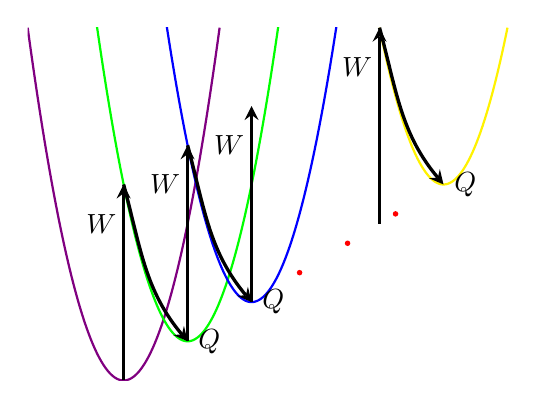
\begin{tikzpicture}
	\def\lims{xmin=-3,xmax=14,ymin=-0.001,ymax=9}
	\begin{axis}[\lims,hide x axis, hide y axis,width=0.7\textwidth,height=0.5\textwidth]
	\addplot[thick,violet,mark=none,samples=1000,domain=-3:3,y domain=-0.001:9] {0+(x-0)*(x-0)};
	\addplot[thick,green,mark=none,samples=1000,domain=-1:5,y domain=-0.001:9] {1+(x-2)*(x-2)};
	\addplot[thick,blue,mark=none,samples=1000,domain=1:7,y domain=-0.001:9] {2+(x-4)*(x-4)};
	\fill[red] (axis cs:5.5,2.75) circle[radius=1pt];
	\fill[red] (axis cs:7,3.5) circle[radius=1pt];
	\fill[red] (axis cs:8.5,4.25) circle[radius=1pt];
	\addplot[thick,yellow,mark=none,samples=1000,domain=8:12,y domain=-0.001:9] {5+(x-10)*(x-10)};
	\draw[very thick,->,>=stealth] (axis cs:0,0) to (axis cs:0,5);
	\draw[very thick,->,>=stealth] (axis cs:2,1) to (axis cs:2,6);
	\draw[very thick,->,>=stealth] (axis cs:4,2) to (axis cs:4,7);
	\draw[very thick,->,>=stealth] (axis cs:8,4) to (axis cs:8,9);
	\draw (axis cs:0-0.7,4) node{$W$};
	\draw (axis cs:2-0.7,5) node{$W$};
	\draw (axis cs:4-0.7,6) node{$W$};
	\draw (axis cs:8-0.7,8) node{$W$};
	\draw[very thick,->,>=stealth] (axis cs:0,5) to [out=285,in=130] (axis cs:2,1) node[right]{$Q$};
	\draw[very thick,->,>=stealth] (axis cs:2,6) to [out=285,in=130] (axis cs:4,2) node[right]{$Q$};
	\draw[very thick,->,>=stealth] (axis cs:8,9) to [out=285,in=130] (axis cs:10,5) node[right]{$Q$};
	
	\end{axis}
	
	\end{tikzpicture}
	\caption{The accumulation of work and heat along a nonequilibrium trajectory. The work is defined as the energy change when the coupling parameter switches from $\lambda_i$ to $\lambda_{i+1}$ with the coordinates fixed, while the dissipated heat is defined as the energy relaxation when the coordinate change with the coupling parameter fixed.}\label{Fig:FEM:NEW}
\end{figure}

%\begin{figure}[htbp]
%	\centering
%	\includegraphics[width=0.4\textwidth]{figures/NEW.pdf}\\
%	\caption{The accumulation of work and heat along a nonequilibrium trajectory. The work is defined as the energy change when the coupling parameter switches from $\lambda_i$ to $\lambda_{i+1}$ with the coordinates fixed, while the dissipated heat is defined as the energy relaxation when the coordinate change with the coupling parameter fixed.}\label{Fig:FEM:NEW}
%\end{figure}

In Ref.~\cite{CrooksJSP1998}, Crooks showed that the distributions of work values from the forward and the backward paths satisfy a relation that is central to the histogram methods in free energy calculations
\begin{equation}
\frac{p_{f}[w=W(\tau)]}{p_{b}[w=-\underline{W}(\tau)]}=\exp[\beta(w-\Delta A)],
\label{Eq:FEM:NEW:crooks}
\end{equation}
where $p_{f}[w=W(\tau)]$ and $p_{b}[w=-\underline{W}(\tau)]$ are the probability densities of the work values in the forward and the reverse transformations (with a sign change for the work in the reverse path). Both are normalized, i.e., $\int p_{f}(w) \diff w=\int p_{b}(w) \diff w=1$. It is noted that Jarzynski equality Eq.~\ref{Eq:FEM:NEW:Jar} follows from Eq.~\ref{Eq:FEM:NEW:crooks} simply by integration over $w$ because the probability densities are normalized to 1:
\begin{equation}
\int p_{f}(W)e^{-\beta W}\diff W=\int p_{b}(W)e^{-\beta \Delta A}\diff W,
\label{Eq:FEM:NEW:crookstojar}
\end{equation}
Because of the normalization condition, the right-hand side is equal to $\exp(-\beta \Delta A)$, and Jarzynski equality follows.

Following the Crooks Fluctuation Theorem (CFT),\cite{CrooksJSP1998} Bennett acceptance ratio can be applicable to nonequilibrium calculations. This approach was combined with a maximum likelihood estimate, and accurate free energy differences were obtained.\cite{ShirtsPRL2003}
In this approach, $\Delta A$ is calculated via
\begin{align}
\sum_{i=1}^{n_{F}}\frac{1}{1+\exp \left[\beta(M+W_{i}-\Delta A)\right]} = \sum_{j=1}^{n_{R}}\frac{1}{1+\exp \left[-\beta(M+W_{j}-\Delta A)\right]},
\label{Eq:FEM:NEW:NEBAR}
\end{align}
where $n_{F}$ and $n_{R}$ are the numbers of the forward and reverse transformations respectively, $W_{i}$ and $W_{j}$ are the work of forward and reverse measurements respectively, and $M=\beta^{-1}$ln($n_{F}$/$n_{R}$).
The corresponding statistical variance of $ \Delta A $, $ \sigma^2 $, is calculated using Eq.~10 in Ref.~\cite{ShirtsPRL2003}.
\clearpage 
% !TeX spellcheck = en_US
% !TeX encoding = UTF-8
\subsection{Transition-Based Reweighting Analysis Method\label{Sec:FEM:TRAM}}
Transition-Based Reweighting Analysis Method (TRAM), which relies on the maximum likelihood analysis of the thermodynamic and kinetic information, was developed by Frank No\'{e} and coworkers in 2014.\cite{WuJCP2014}. It incorporates WHAM with Markov state model, and avoids the weakness in both methods. In WHAM, a global equilibrium among all the thermodynamic states must be reached. For the Markov state model (MSM), the kinetic information can be extracted from only one thermodynamic state. In contrast, TRAM is a class of estimators that (1) takes the statistical weights of samples at different thermodynamic states into account, and (2) exploits transitions observed in the sampled trajectories, without assuming that these trajectories are sampled from equilibrium.

Let us assume that there are $K$ molecular dynamics (MD) or Markov chain Monte Carlo (MCMC) simulations have been performed, each in a specific thermodynamic state (Hamiltonian, temperature, etc) indexed by $k\in \{1,\dots,K\}$. For simulations with varying thermodynamic state in a single trajectory, with replica-exchange simulation being a typical example, each contiguous sequence is treated as a separated trajectory at one of the $K$ thermodynamic states. We further assume the configuration space (that has been visited by the simulations) is discretized into cells indexed by $i,j\in \{1,\dots,n\}$. 

Similar to the WHAM analysis, the unbiased probability, $\pi_i$, and the biased probability under thermodynamic state $k$, $\pi_i^{(k)}$ are related by a known and constant bias factor $\gamma_i^{(k)}$
\begin{align}
    \pi_i^{(k)}=f^{(k)}\pi_i\gamma_i^{(k)},\label{Eq:FEM:TRAM:reweight}\\
    f^{(k)}=\frac{1}{\sum_l \pi_l\gamma_l^{(k)}}\label{Eq:FEM:TRAM:f},
\end{align}
where $f^{(k)}$ is a normalization constant. Thus, the bias is multiplicative in probability or additive in the potential. As we have shown in section~\ref{Sec:FEM:WHAM}, the WHAM estimator can be derived by maximizing the likelihood
\begin{equation}
    L_{WHAM}=\prod\limits_k\prod\limits_i (\pi_i^{(k)})^{N_i^{(k)}}
\end{equation}
with an implied assumption that every count $N_i^{(k)}$ is independently drawn from the biased distribution $\pi_i^{(k)}$.

The maximum likelihood Markov model is the transition matrix $\mathbf{P}=(p_{ij})$ between $n$ discrete configuration states, that maximizes the likelihood of the observed transitions between these states. The likelihood of a Markov model is a product of all transition probabilities corresponding to the observed trajectory. To obtain a reversible Markov state model, this likelihood is maximized under the constraints of detailed balance with respect to the equilibrium distribution $\boldsymbol{\pi}$
\begin{align}
    L_{MSM}=\prod_i\prod_j p_{ij}^{c_{ij}},\\
    s.t.\quad \pi_i p_{ij}=\pi_j p_{ji} \quad \text{for all} i,j,
\end{align}
where $c_{ij}$ is the number of times the trajectories were observed in state $i$ at time $t$ and in state $j$ at a later time $t+\tau$, where $\tau$ is the lag time at which the Markov model is estimated.

In TRAM, WHAM and MSM are combined as follows: every trajectory at thermodynamic state $k$ is treated as a Markov chain with the configuration-state transition counts $c_{ij}^{(k)}$, without assuming that every count is sampled from global equilibrium. In contrast to Markov models, we exploit the fact that equilibrium probabilities can be reweighted between different thermodynamic states via Eqs.~\ref{Eq:FEM:TRAM:reweight} and~\ref{Eq:FEM:TRAM:f}. The resulting likelihood of all $\mathbf{P}^{(k)}$ and $\boldsymbol{\pi}$, based on simulations at all thermodynamic states can be formulated as
\begin{align}
	L_{TRAM}=\prod_k\prod_i\prod_j (p_{ij}^{(k)})^{c_{ij}^{(k)}},\label{Eq:FEM:TRAM:TRAMlikelihood}\\
	s.t.\quad \pi_i^{(k)}p_{ij}^{(k)}=\pi_j^{(k)}p_{ji}^{(k)}\quad \text{for all }i,j,k. \label{Eq:FEM:TRAM:TRAMdetailedbalance}
\end{align}
Here, $\mathbf{P}^{(k)}=(p_{ij}^{(k)})$ is the Markov transition matrix at thermodynamic state $k$, and $c_{ij}^{(k)}$ are the number of transitions observed at that simulation condition. $\boldsymbol{\pi}^{(k)}$ is the vector of equilibrium probabilities of discrete states at each thermodynamic state. \emph{Because each Markov model $\mathbf{P}^{(k)}$ must have the distribution $\boldsymbol{\pi}^{(k)}$ as a stationary distribution, all Markov models are coupled too, which makes the maximization of the TRAM likelihood Eqs.~\ref{Eq:FEM:TRAM:TRAMlikelihood} and~\ref{Eq:FEM:TRAM:TRAMdetailedbalance} difficult, and it can neither be achieved by WHAM, nor by existing MSM estimators.}

Taking natural logarithm on the TRAM likelihood, we find
\begin{equation}
    \ln{L_{TRAM}}=\sum_{k=1}^{K}\sum_{i=1}^n\sum_{j=1}^{n}c_{ij}^{(k)}\ln{p_{ij}^{(k)}},
\end{equation}
with constraints
\begin{equation}
    \pi_i\gamma_i^{(k)}p_{ij}^{(k)}=\pi_j\gamma_j^{(k)}p_{ji}^{(k)}\quad \text{for all }i,j,k,
\end{equation}
which is from Eqs.~\ref{Eq:FEM:TRAM:reweight} and~\ref{Eq:FEM:TRAM:TRAMdetailedbalance} with $f^{(k)}$ canceled. In addition, $\mathbf{P}^{(k)}$ and $\boldsymbol{\pi}$ should satisfy the normalization conditions
\begin{align}
	\sum_{j}p_{ij}^{(k)}=1 \quad \forall i,k,\\
	\sum_j \pi_j=1.
\end{align}
The normalization of $\boldsymbol{\pi}^{(k)}$ is naturally satisfied due to Eqs.~\ref{Eq:FEM:TRAM:reweight} and~\ref{Eq:FEM:TRAM:f}. Due to the existence of constraints, the numbers of free variables are $n-1$ for $\boldsymbol{\pi}$ and $n(n-1)/2$ for $\mathbf{P}^{(k)}$.

Using the Lagrange duality theory, it can be shown that the optimal solution of the discrete TRAM problem above fulfills the following two conditions
\begin{align}
	\sum_k\sum_j\frac{(c_{ij}^{(k)}+c_{ji}^{(k)})\gamma_i^{(k)}\pi_i\nu_j^{(k)}}{\gamma_i^{(k)}\pi_i\nu_j^{(k)}+\gamma_j^{(k)}\pi_j\nu_i^{(k)}}=\sum_k\sum_jc_{ji}^{(k)},\\
	\sum_j\frac{(c_{ij}^{(k)}+c_{ji}^{(k)})\gamma_j^{(k)}\pi_j}{\gamma_i^{(k)}\pi_i\nu_j^{(k)}+\gamma_j^{(k)}\pi_j\nu_i^{(k)}}=1
\end{align}
where $\nu_i^{(k)}$ are unknown Lagrange multipliers. To numerically solve the discrete TRAM problem, an initial guess for $\boldsymbol{\pi}$ and $\mathbf{v}^{(k)}$ can be made as
\begin{align}
	\pi_i^{init}:=1/n,
	v_i^{(k),init}:=\sum_j c_{ij}^{(k)},
\end{align}
and the following equations must be solved iteratively until $\boldsymbol{\pi}$ is converged:
\begin{align}
	v_i^{(k),new}:=v_i^{(k)}\sum_j \frac{(c_{ij}^{(k)}+c_{ji}^{(k)})\gamma_i^{(k)}\pi_j}{\gamma_i^{(k)}\pi_i\nu_j^{(k)}+\gamma_j^{(k)}\pi_j\nu_i^{(k)}},\\
	\pi_i^{new}:=\frac{\sum_{k,j}c_{ji}^{(k)}}{\sum_{k,j}\frac{(c_{ij}^{(k)}+c_{ji}^{(k)})\gamma_i^{(k)}\nu_j^{(k)}}{\gamma_i^{(k)}\pi_i\nu_j^{(k)}+\gamma_j^{(k)}\pi_j\nu_i^{(k)}}}.
\end{align}
\clearpage 
% !TeX spellcheck = en_US
\subsection{Normalizing Flow\label{Sec:FEM:NF}}
In 2002, Jarzynski proposed a generalized free energy perturbation method termed ``targeted free energy perturbation''.\cite{JarzynskiPRE2002} This method generalizes the free energy perturbation method between two states, $A$ and $B$, by introducing an intermediate state $A^\prime(\mathbf{y})$ by mapping $\mathcal{M}$ from the microstate of the system $\mathbf{x}$ to another one $\mathbf{y}$ in the configuration space or phase space
\begin{equation}
	\mathcal{M}: \mathbf{x} \to \mathbf{y}(\mathbf{x}),
\end{equation}
The potential energy function of the mapped state $A^\prime(\mathbf{y})$ is
\begin{equation}
	U_{A^\prime}(\mathbf{y})=U_A(\mathbf{x})+\beta^{-1}\ln J(\mathbf{x}),
\end{equation}
where $J(\mathbf{x})=|\partial \mathbf{y}/\partial \mathbf{x}|$ is the Jacobian of the mapping $\mathcal{M}$. Zhu et al also used this transformation, but for enhancing conformational sampling.\cite{ZhuPRL2002} The Helmholtz free energy difference between state $A$ and state $A^\prime$ is zero by noticing that
\begin{align*}
	\Delta F_{A^\prime A}=&-\beta^{-1}\ln\frac{Z_{A^\prime}}{Z_A}\notag\\
	=&-\beta^{-1}\ln \frac{\displaystyle\int e^{-\beta U_{A^\prime}(\mathbf{y})}\diff y}{Z_A}\notag\\
	=&-\beta^{-1}\ln \frac{\displaystyle\int e^{-\beta (U_{A^\prime}(\mathbf{y})-U_A(\mathbf{x}))}e^{-\beta U_A(\mathbf{x})}\diff y}{Z_A}\notag\\
	=&-\beta^{-1}\ln \frac{\displaystyle\int J^{-1}(\mathbf{x})e^{-\beta U_A(\mathbf{x})}\diff y}{Z_A}\notag\\
	=&-\beta^{-1}\ln \frac{\displaystyle\int e^{-\beta U_A(\mathbf{x})}\diff x}{Z_A}\notag\\
	=&0.
\end{align*}
The calculation of the free energy difference between state $A$ and state $B$ can be replaced by the calculation of free energy difference between state $A^\prime$ and state $B$. The latter can be written as
\begin{align}
	\Delta F_{BA^\prime}=&-\beta^{-1}\ln {\int e^{-\beta (U_B(\mathbf{y})-U_{A^\prime}(\mathbf{y}))}\rho_{A^\prime}(\mathbf{y})\diff \mathbf{y}}\notag\\
	=&-\beta^{-1}\ln {\int e^{-\beta \Phi(\mathbf{x})}\rho_{A}(\mathbf{x})\diff \mathbf{x}}
\end{align}
in which 
\begin{align}
	\Phi(\mathbf{x})\equiv& U_B(\mathbf{y}) - U_{A^\prime}(\mathbf{y})\notag\\
	=&U_B(\mathbf{y})-U_A(\mathbf{x})-\beta^{-1}\ln J(\mathbf{x}),
	\label{Eq:FEM:TP:TFEPPhi}
\end{align}
and the relationship between the distributions
\begin{equation}
	\rho_{A^\prime}(\mathbf{y})=\rho_{A}(\mathbf{x})/J(\mathbf{x})
	\label{Eq:FEM:TP:TFEPdistribution}
\end{equation}
has been invoked.

As a special case $\mathcal{M}: \mathbf{x} \to\mathbf{x}$,
\begin{equation}
	\Phi(\mathbf{x})\equiv U_B(\mathbf{x})-U_A(\mathbf{x}),
\end{equation}
and it reduces to the traditional free energy perturbation. It implies that there may exist an invertible mapping $\mathcal{M}$ for which the average of $\exp\{-\beta \Phi\}$ converges more rapidly than the average of $\exp\{-\beta (U_B-U_A)\}$. It can also be asserted that
\begin{align}
	e^{-\beta \Delta F}=&\left<e^{-\beta \Phi}\right>_A\notag\\
	=&\int \diff \mathbf{x}\, \rho(\mathbf{x})e^{-\beta \Phi(\mathbf{x})}\notag\\
	=&\int \diff\phi \int \diff \mathbf{x}\, \rho(\mathbf{x})e^{-\beta \Phi(\mathbf{x})}\delta(\Phi(\mathbf{x})-\phi)\notag\\
	=&\int \diff\phi\, e^{-\beta \phi}\int \rho(\mathbf{x})\delta(\Phi(\mathbf{x})-\phi)\diff \mathbf{x}\notag\\
	=&\int \diff\phi\, e^{-\beta \phi} p(\phi|\mathcal{M}),
\end{align}
where $p(\phi|\mathcal{M})$ is the distribution of values of $\phi=\Phi(\mathbf{x})$ for $\mathbf{x}$ sampled from $A$. In practice, $\Delta F$ can be estimated by averaging $\exp{(-\beta \Phi)}$ over a finite number of sampled microstates $\mathbf{x}_1,\,\mathbf{x}_2,\dots,\mathbf{x}_N$
\begin{equation}
	\Delta F=-\beta^{-1}\ln\frac{1}{N}\sum_{n=1}^N e^{-\beta \Phi(\mathbf{x}_n)}.
\end{equation}
The rate of convergence depends on the choice of $\mathcal{M}$. With a perfect mapping $\mathcal{M}^\ast$ that transforms $A$ exactly onto $B$, we will find from Eq.~\ref{Eq:FEM:TP:TFEPdistribution} that
\begin{equation}
	\frac{1}{Z_B}e^{-\beta U_B(\mathbf{y})}=\frac{1}{Z_A}e^{-\beta U_A(\mathbf{x})}/J(\mathbf{x}).
\end{equation}
By taking it into Eq.~\ref{Eq:FEM:TP:TFEPPhi}, we will have
\begin{equation}
	\Phi(\mathbf{x})=\Delta F,
\end{equation}
which means
\begin{equation}
	p(\phi|\mathcal{M}^\ast)=\delta (\phi-\Delta F).
\end{equation}
Then the convergence of the finite sampling is immediate: $\Phi(\mathbf{x})=\Delta F$ for every sampled $\mathbf{x}$. Although constructing a perfect transformation is usually impossible for real-world problems, a transformation that keeps a narrow distribution of $\phi$'s, which implies good overlap between the transformed state and state $B$, can accelerate the convergence of the generalized free energy perturbation calculations.

Recently, Rizzi et al. showed that if the samples are used for both the optimization/learning of the mapping, it will cause systematic error in the calculated free energy change.\cite{RizziJPCL2021} They suggested to use a small data set for learning and a large set for evaluating the free energy change.

In 2009, Hahn and Then extended this idea and proposed a bidirectional formulation as a generalized Bennett Acceptance Ratio method\cite{HahnPRE2009}.
They began with the identity, which can be easily obtained from Eq.~\ref{Eq:FEM:TP:TFEPPhi},
\begin{equation}
	\frac{\rho_{A^\prime}(\mathbf{y}(\mathbf{x}))}{\rho_B(\mathbf{y}(\mathbf{x}))}=e^{\beta\left[\Phi(\mathbf{x})-\Delta F\right]}\qquad \forall \mathbf{x}\in \Gamma_A.
\end{equation}
Multiplying both sides with $\delta [W-\Phi(\mathbf{x})]\rho_B(\mathbf{y}(\mathbf{x}))$ and integrating with respect to $\mathbf{y}$, the left-hand side yields
\begin{align}
	\int_{\mathbf{y}(\Gamma_A)}&\delta[W-\Phi(\mathbf{x})]\rho_{A^\prime}(\mathbf{y}(\mathbf{x}))\diff \mathbf{y}\notag\\
	=&\int_{\Gamma_A}\delta[W-\Phi(\mathbf{x})]\rho_A(\mathbf{x})\diff \mathbf{x}\notag\\
	=&p(W|A;\mathcal{M}),
\end{align}
and the right-hand side yields
\begin{align}
	\int_{\mathbf{y}(\Gamma_A)}&e^{\beta\left[\Phi(\mathbf{x})-\Delta F\right]}\delta[W-\Phi(\mathbf{x})]\rho_B(\mathbf{y})\diff \mathbf{y}\notag\\
	=&e^{\beta\left[W-\Delta F\right]}\int_{\mathbf{y}(\Gamma_A)}\delta[W-\Phi(\mathbf{x})]\rho_B(\mathbf{y})\diff \mathbf{y}\notag\\
	=&e^{\beta\left[W-\Delta F\right]}p(W|B;\mathcal{M}),
\end{align}
where $p(W|A;\mathcal{M})$ ($p(W|B;\mathcal{M})$) is the probability density for the outcome of a specific value of the generalized work $W$ in forward (reverse) direction subject to the map $\mathcal{M}$ when sampled from $\rho_A$ ($\rho_B$). Then, we arrive at the fluctuation theorem for any differentiable, bijective map $\mathcal{M}$ from $\Gamma_A$ to $\Gamma_B$
\begin{equation}
	\frac{p(W|A;\mathcal{M})}{p(W|B;\mathcal{M})}=e^{\beta\left[W-\Delta F\right]}.
	\label{Eq:FEM:TP:FluctTheo}
\end{equation}
Bayes theorem,
\begin{equation}
	p(W|Y)p_Y=p(Y|W)p(W), \quad \text{with $Y=A$ or $B$}
	\label{Eq:FEM:TP:Bayes}
\end{equation}
implies the ``balance'' equation
\begin{align}
	p_B\int p(A|W)p(W|B)\diff W=&\int p(A|W)p(B|W)p(W)\diff W\notag\\
	=&\int p(B|W)p(W|A)p_A\diff W\notag\\
	=&p_A\int p(B|W)p(W|A)\diff W,
	\label{Eq:FEM:TP:BalEq}
\end{align}
or $p_B\left<p(A|W)\right>_B=p_A\left<p(B|W)\right>_A$.

Combining Eq.~\ref{Eq:FEM:TP:FluctTheo} and Eq.~\ref{Eq:FEM:TP:Bayes} leads to
\begin{equation}
	\frac{p(A|W)}{p(B|W)}=e^{\beta(W-C)}
\end{equation}
with
\begin{equation}
	C=\Delta F+\frac{1}{\beta}\ln{\frac{p_B}{p_A}}.
\end{equation}
With the normalization condition $p(A|W)+p(B|W)=1$, it yields
\begin{equation}
	p(A|W)=\frac{1}{1+e^{\beta(C-W)}}
\end{equation}
and
\begin{equation}
	p(B|W)=\frac{e^{\beta(C-W)}}{1+e^{\beta(C-W)}}=\frac{1}{1+e^{\beta(-C+W)}}.
\end{equation}
Replacing both, the ensemble averages by sample averages and the ratio $\frac{p_B}{p_A}$ by $\frac{n_B}{n_A}$, the balance equation Eq.~\ref{Eq:FEM:TP:BalEq} results in
\begin{equation}
	\sum_{j=1}^{n_B}\frac{1}{1+\frac{n_B}{n_A}\exp{\left(\beta\widehat{\Delta F}_{AB}-\beta W^j_B\right)}}=	\sum_{i=1}^{n_A}\frac{1}{1+\frac{n_B}{n_A}\exp{\left(-\beta\widehat{\Delta F}_{AB}+\beta W^i_A\right)}}.
\end{equation}
They also suggested using Kullback-Leibler divergence to characterize the similarity between the mapped state $A^\prime$ and state $B$.

Paliwal and Shirts combined this idea of mapping in configurational space with MBAR.\cite{PaliwalJCP2013}

Ding and Zhang further extended this idea and integrated BAR with a deep generative model and developed an efficient free energy method DeepBAR.\cite{DingJPCL2021}
\section{Approximate Methods}
% !TeX spellcheck = en_US
\subsection{Molecular Mechanics/Poisson-Boltzmann Surface Area\label{Sec:FEM:MMPBSA}}
The following derivation follows Ref.~\cite{SwansonBJ2004}.
The Molecular Mechanics/Poisson-Boltzmann Surface Area (MM/PBSA) method is often used in the calculations of binding free energy of a substrate to a receptor.
The standard binding free energy for a reaction between a receptor (A) and a substrate (B)
\begin{equation}
	A\,+\,B\rightleftharpoons AB
\end{equation}
is expressed as a ratio of configuration integrals
\begin{align}
	\Delta G_{AB}^0 =& -RT\ln{\left(\frac{C^0}{8\pi^2}\cdot\frac{Z_{N,AB}Z_{N,0}}{Z_{N,A}Z_{N,B}}\right)}+P^0\left<\Delta V_{AB}\right>\notag\\
	                =& -RT\ln{\left(\frac{C^0}{8\pi^2}\cdot\frac{\frac{Z_{N,AB}}{Z_{N,0}}}{\frac{Z_{N,A}}{Z_{N,0}}\frac{Z_{N,B}}{Z_{N,0}}}\right)}+P^0\left<\Delta V_{AB}\right>,
	\label{Eq:FEM:MMPBSA:deltaG}
\end{align}
where R is the gas constant, T is the temperature, $C^0$ is the standard state concentration (1 $M$), $N$ is the number of solvent molecules, and $P^0\left<\Delta V_{AB}\right>$ is the pressure-volume work associated with changing the system size after the association of two species into one complex. For water solution at 1 atm, the last term is negligibly small. There are no mass-dependent terms in Eq.~\ref{Eq:FEM:MMPBSA:deltaG}, which is a direct result of equal kinetic contribution to the partition function of the bound and the free species. The configuration integral of the receptor, A, in solution is
\begin{equation}
	Z_{N,A}=\int e^{-\beta U(r_A,r_S)}dr_Adr_S,
\end{equation}
where $U(r_A,r_S)$ is the potential energy as a function of all solute coordinates, $r_A$, and solvent coordinates, $r_S$, and $\beta$ is the reciprocal of the product of the Boltzmann constant and temperature. The total potential energy can be decomposed into $U(r_A)+U(r_S)+\Delta U(r_A,r_S)$. Similar for $B$, the substrate. For pure solvent, the configuration integral is
\begin{equation}
	Z_{N,0}=\int e^{-\beta U(r_S)}dr_S.
\end{equation}
The ratio of configuration integrals in Eq.~\ref{Eq:FEM:MMPBSA:deltaG} can be simplified with an implicit solvent approximation, as
\begin{align}
	\frac{Z_{N,A}}{Z_{N,0}}=Z_A=&\frac{\int e^{-\beta U(r_A)}\left\{\int e^{-\beta\Delta U(r_A,r_S)}e^{-\beta U(r_S)}dr_S\right\}dr_A}{\int e^{-\beta U(r_S)}dr_S}\notag\\
	                           =&\int e^{-\beta \left[U(r_A)+W(r_A)\right]}dr_A,
\end{align}
where
\begin{equation}
	W(r_A)=-RT\ln{\left(\frac{\int e^{-\beta\Delta U(r_A,r_S)}e^{-\beta U(r_S)}dr_S}{\int e^{-\beta U(r_S)}dr_S}\right)}
\end{equation}
is the solvation free energy of the receptor $A$ at fixed coordinate $r_A$. Analogous equations hold for the complex and substrate.

For the complex, we define the position (translational degrees of freedom) and orientation (rotational degrees of freedom) of the substrate with respective to the receptor as $\delta_B\equiv\left(x_1,x_2,x_3,\xi_1,\xi_2,\xi_3\right)$. Generally, these degree-of-freedom is very limited. The complex configuration integral is 
\begin{equation}
	Z_{AB}=\int e^{-\beta\left[U\left(r_A,r_{B^\prime},\delta_B\right)+W\left(r_A,r_{B^\prime},\delta_B\right)\right]}dr_Adr_{B^\prime}d\delta_B,
\end{equation}
where $r_{B^\prime}$ represents the remaining internal degrees of freedom of the bound substrate and $\delta_B$ spans conformations where $A$ and $B$ form a complex. 
Then we assume that the translational and rotational motions of the substrate in the bound state are not strongly coupled with the other degrees of freedom, and we decompose the potential and solvation energies as (\textit{so weird!})
\begin{align}
	U&\left(r_A,r_{B^\prime},\delta_B\right)+W\left(r_A,r_{B^\prime},\delta_B\right)\notag\\
	 &\approx U_1(\delta_B) + W_1(\delta_B) +U_2(r_A,r_{B^\prime})+W_2(r_A,r_{B^\prime}).
\end{align}
We further assume that the residual translational and rotational motions of the substrate are uncorrelated. Therefore
\begin{equation}
	U_1(\delta_B) \approx U(x_1,x_2,x_3) + U(\xi_1,\xi_2,\xi_3),
\end{equation}
and
\begin{equation}
	W_1(\delta_B) \approx W(x_1,x_2,x_3) + W(\xi_1,\xi_2,\xi_3).
\end{equation}

Now, Eq.~\ref{Eq:FEM:MMPBSA:deltaG} can bre written as
\begin{equation}
   \Delta G_{AB}^0=-RT\ln{\left[\frac{C^0Z_{B^\prime}^{trans}Z_{B^\prime}^{rot}Z_{AB^\prime}}{8\pi^2Z_AZ_B}\right]},
\end{equation}
where
\begin{equation}
   Z_{B^\prime}^{trans}=\int e^{-\beta\left[U(x_1,x_2,x_3)+W(x_1,x_2,x_3)\right]}dx_1dx_2dx_3
\end{equation}
and
\begin{equation}
	Z_{B^\prime}^{rot}=\int e^{-\beta\left[U(\xi_1,\xi_2,\xi_3)+W(\xi_1,\xi_2,\xi_3)\right]}d\xi_1d\xi_2d\xi_3.
\end{equation}
As a first-order approximation, we assume that the energetic landscape of each species has an energy and a volume (entropy),
\begin{equation}
	Z_A=\int e^{-\beta \left[U(r_A)+W(r_A)\right]}dr_A\approx Z_A^{int}e^{-\beta \left<E_A\right>},
\end{equation}
where $\left<E_A\right>=\left<U(r_A)+W(r_A)\right>$. We further assume (\textit{how many approximations we have taken!}) that $Z_A^{int}Z_B^{int}\approx Z_{AB}^{int}$,
then
\begin{equation}
	\Delta G_{AB}^0=-RT\ln{\left(\frac{C^0Z_{B^\prime}^{trans}Z_{B^\prime}^{rot}}{8\pi^2}\right)} +\left(\left<E_{AB^\prime}\right>-\left<E_A\right>-\left<E_B\right>\right).
\end{equation}
 
The bound substrate's translational configuration integral, $Z_{B^\prime}^{trans}$, can be conceptually linked to the volume of space that its center of mass occupies through the simulation. The effective volume was measured based on the assumption that the translational motion is restrained by three harmonic potential. By solving eigenstates of the center-of-mass covariance matrix, the eigenvalues describe the variance $\Delta x_i^2$ along each principal axis. Thus, the translational configuration integral can be calculated as
\begin{align}
Z_{B^\prime}^{trans}=&\int e^{\left(-k_1\Delta x_1^2/2k_BT\right)}dx_1\int e^{\left(-k_2\Delta x_2^2/2k_BT\right)}dx_2\int e^{\left(-k_3\Delta x_3^2/2k_BT\right)}dx_3\notag\\
                    =&(2\pi)^{3/2}\left(\left<\Delta x_1^2\right>\left<\Delta x_2^2\right>\left<\Delta x_3^2\right>\right)^{1/2}
\end{align}
where
\begin{equation}
k_i=\frac{k_B T}{\left<\Delta x_i^2\right>}.
\end{equation}
The rotational configuration integral can be accounted in a similar manner.